{\centering \nonumsubsection{A \hspace{1em} 组}}
\begin{xiaotis}

\xiaoti{下面的说法正确吗? 为什么?}
\begin{xiaoxiaotis}

    \xxt{两条直线确定一个平面;}

    \xxt{如果两个平面有三个公共点,那么这两个平面重合。}

\end{xiaoxiaotis}


\xiaoti{}%
\begin{xiaoxiaotis}%
    \xxt[\xxtsep]{求证:两两相交且不共点的四条直线共面;}

    \xxt{已知四个点不共面,证明它们中任何三点都不在同一条直线上。逆命题正确吗?}

\end{xiaoxiaotis}


\xiaoti{用斜二例画法画出下列水平放置的图形的直观图。}

\begin{figure}[htbp]
    \centering
    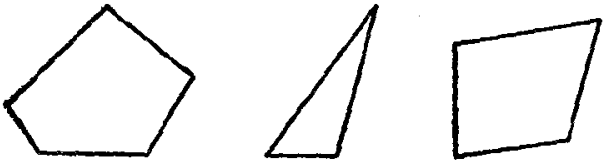
\includegraphics[width=7cm]{../pic/ltjh-ch1-fuxi-03.png}
    \caption*{(第 3 题)}
\end{figure}

\xiaoti{}%
\begin{xiaoxiaotis}%
    \xxt[\xxtsep]{已知 $a$ 和 $b$ 是异面直线, $a$ 和 $c$ 是异面直线,那么 $b$ 和 $c$ 也是异面直线吗?}

    \xxt{在一个平面内,经过一条直线外一点有几条直线和这条直线垂直?在空间呢?}

    \xxt{在一个平面内,经过一条直线外一点有几条直线和这条直线平行?在空间呢?}

\end{xiaoxiaotis}


\xiaoti{求证:过两条平行线中一条直线的所有平面,与另一条直线平行或经过另一条直线。}

\xiaoti{如果一条直线上的两点在一个平面的同侧,并且和这个平面的距离相等,那么这条直线和平面平行。}

\xiaoti{一条直线和一组平行平面中每一个平面所成的角都相等。}

\xiaoti{$Rt \triangle ABC$ 所在平面外一点 $P$ 到直角顶点 $C$ 的距离为 24 cm,到两直角边的距离为 $6\sqrt{10}$ cm。
    求:(1)点 $P$ 到平面 $ABC$ 的距离; (2)$PC$ 与平面所成的角。
}

\xiaoti{正方形的边长为 $a$,中心是 $O$, $OA$ 垂直于正方形所在的平面, $OA$ 的长是 $b$。 求点 $A$ 到正方形各边的距离。}

\xiaoti{三个平面两两相交,有三条交线。求证:这三条交线交于一点或互相平行。}

\xiaoti{夹在两个平行平面之间的两条线段 $AB$、$CD$ 相交于点 $S$, 已知: $AS = 18.9$ cm,
    $BS = 29.4\;\limi$, $CD = 57.5$ cm。 求线段 $CS$、$DS$ 的长。% BS 处使用 \limi 而不是 cm 是为了不将 'cm' 换行显示。其它地方直接使用 cm 是为了省事。
}

\xiaoti{在直二面角的棱上有两点 $A$、$B$, $AC$ 和 $BD$ 各在这个二面角的一个面内,并且都垂直于棱 $AB$。
    设 $AB = 8$ cm, $AC = 6$ cm, $BD = 24$ cm。 求 $CD$ 的长。
}

\xiaoti{已知一个直角三角形的两直角边长为 $a$、$b$,把这个三角形沿斜边上的高折成直二面角。
    求两直角边夹角的余弦。
}

\begin{figure}[htbp]
    \centering
    \begin{minipage}[b]{7cm}
        \centering
        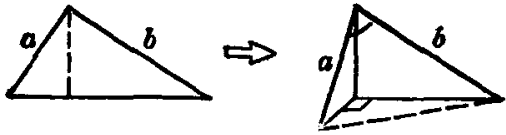
\includegraphics[width=6cm]{../pic/ltjh-ch1-fuxi-13.png}
        \caption*{(第 13 题)}
    \end{minipage}
    \qquad
    \begin{minipage}[b]{7cm}
        \centering
        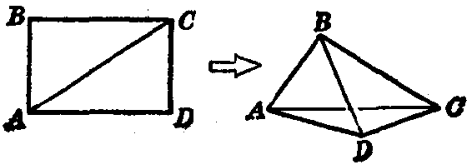
\includegraphics[width=6cm]{../pic/ltjh-ch1-fuxi-14.png}
        \caption*{(第 14 题)}
    \end{minipage}
\end{figure}

\xiaoti{把长、宽各为 4、3 的长方形 $ABCD$ 沿对角线 $AC$ 折成直二面角。 求顶点 $B$ 和 $D$ 的距离。}

\end{xiaotis}
